\startcontents[localtoc]
\printcontents[localtoc]{}{0}{\subsection*{Contents}\setcounter{tocdepth}{2}}



\phantomsection
\addcontentsline{toc}{section}{Set acquisition properties}
\subsubsection*{Set acquisition properties}



First acquisition quantities are prepared: sampling frequency \texttt{fs} set to
10 kHz, and length of the record \texttt{L} set to 1000, representing 0.1 s long record.

\begin{lstlisting}
DI = [];
DI.fs.v = 1e4;
DI.L.v = 1e3;
\end{lstlisting}


\phantomsection
\addcontentsline{toc}{section}{Set waveform properties}
\subsubsection*{Set waveform properties}



The actual waveform will consist of 3 signal components. Main signal
component frequency will be 50 Hz, amplitude 1 V. Third harmonic amplitude
will be set to 0.15 V. Last component will be interharmonic of frequency 79 Hz and amplitude of 0.1 V.

\begin{lstlisting}
DI.f.v =  [50  150 757];
DI.A.v =  [ 1 0.15 0.05];
DI.ph.v = [ 0    0   0];
\end{lstlisting}


\phantomsection
\addcontentsline{toc}{section}{Call algorithm}
\subsubsection*{Call algorithm}



Use QWTB to apply algorithm \texttt{WaveformGenerator} to data \texttt{DI}.

\begin{lstlisting}
CS.verbose = 1;
DO = qwtb('WaveformGenerator', DI, CS);
\end{lstlisting}
\begin{lstlisting}[language={},xleftmargin=5pt,frame=none]
QWTB: no uncertainty calculation

\end{lstlisting}


\phantomsection
\addcontentsline{toc}{section}{Display results}
\subsubsection*{Display results}



Results are the time stamps and samples.

\begin{lstlisting}
plot(DO.t.v, DO.y.v, '-+')
xlabel('t (s)')
title('Waveform generated by WaveformGenerator algorithm')
\end{lstlisting}
\begin{center}
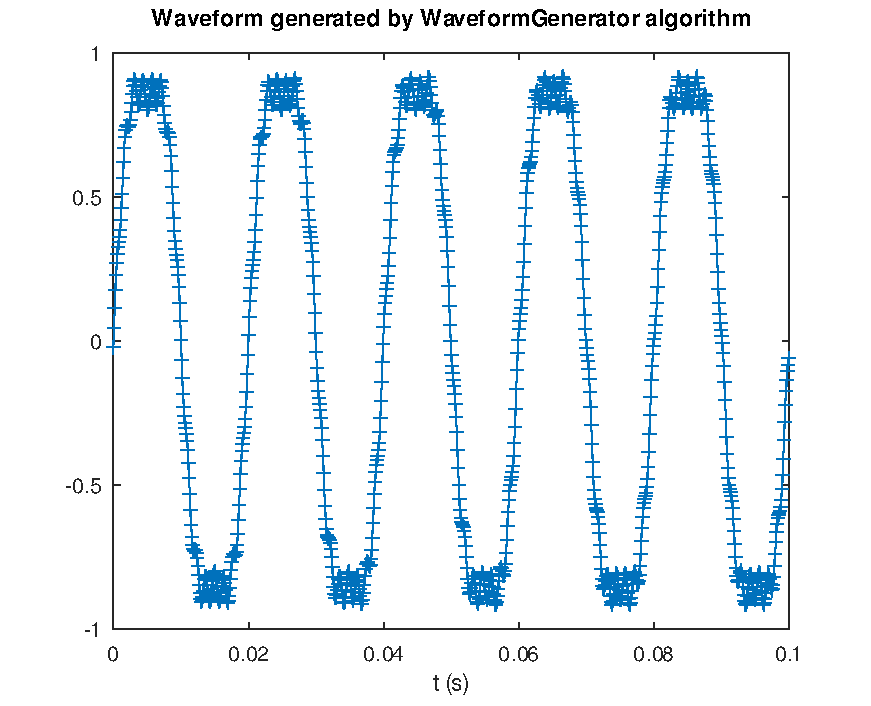
\includegraphics[width=0.7\textwidth]{algs_examples_published/WaveformGenerator_alg_example-1.pdf}
\end{center}


\stopcontents[localtoc]
